
\begin{definition} [Conjunto de nivel] 
\label{def:conjunto de nivel}
 \mbox{}
 
Sea $f: U\subset\Rn{n}\rightarrow\R$ y sea $C\subseteq\R$. Entonces el conjunto de nivel del valor c se define como aquellos puntos $x\in\ U$ para las cuales $f(x)=c$. Si $n=2$ hablamos de curva de nivel (del valor c) y si $n=3$, hablamos de superficie de nivel y se nota, $C(c,f)$, tal que:

 \[
C(c,f)=\{(x_1,x_2,...,x_n) \in U \backslash f (x_1,...,x_n)=c \}
 \]

En primer lugar, se empieza definiendo curva de nivel, donde se toma n=2.
 \[
C(c,f)=\{(x,y) \in U \backslash f (x,y)=c \}
 \]

Ejemplo 1: Se toma la funcion $f(x,y)=x^2+y^2$, donde empezamos a analizar los distintos conjuntos de nivel, tomando $c$ como diferentes constantes
 \[
C(0,f)=\{(x,y) \in U \backslash x^2+y^2=0 \}
\]
 \[
C(1,f)=\{(x,y) \in U \backslash x^2+y^2=1 \}
\]
 \[
C(4,f)=\{(x,y) \in U \backslash x^2+y^2=4 \}
 \]

\begin{figure}[h!] % El entorno figure te permite incluir imágenes
    \centering
    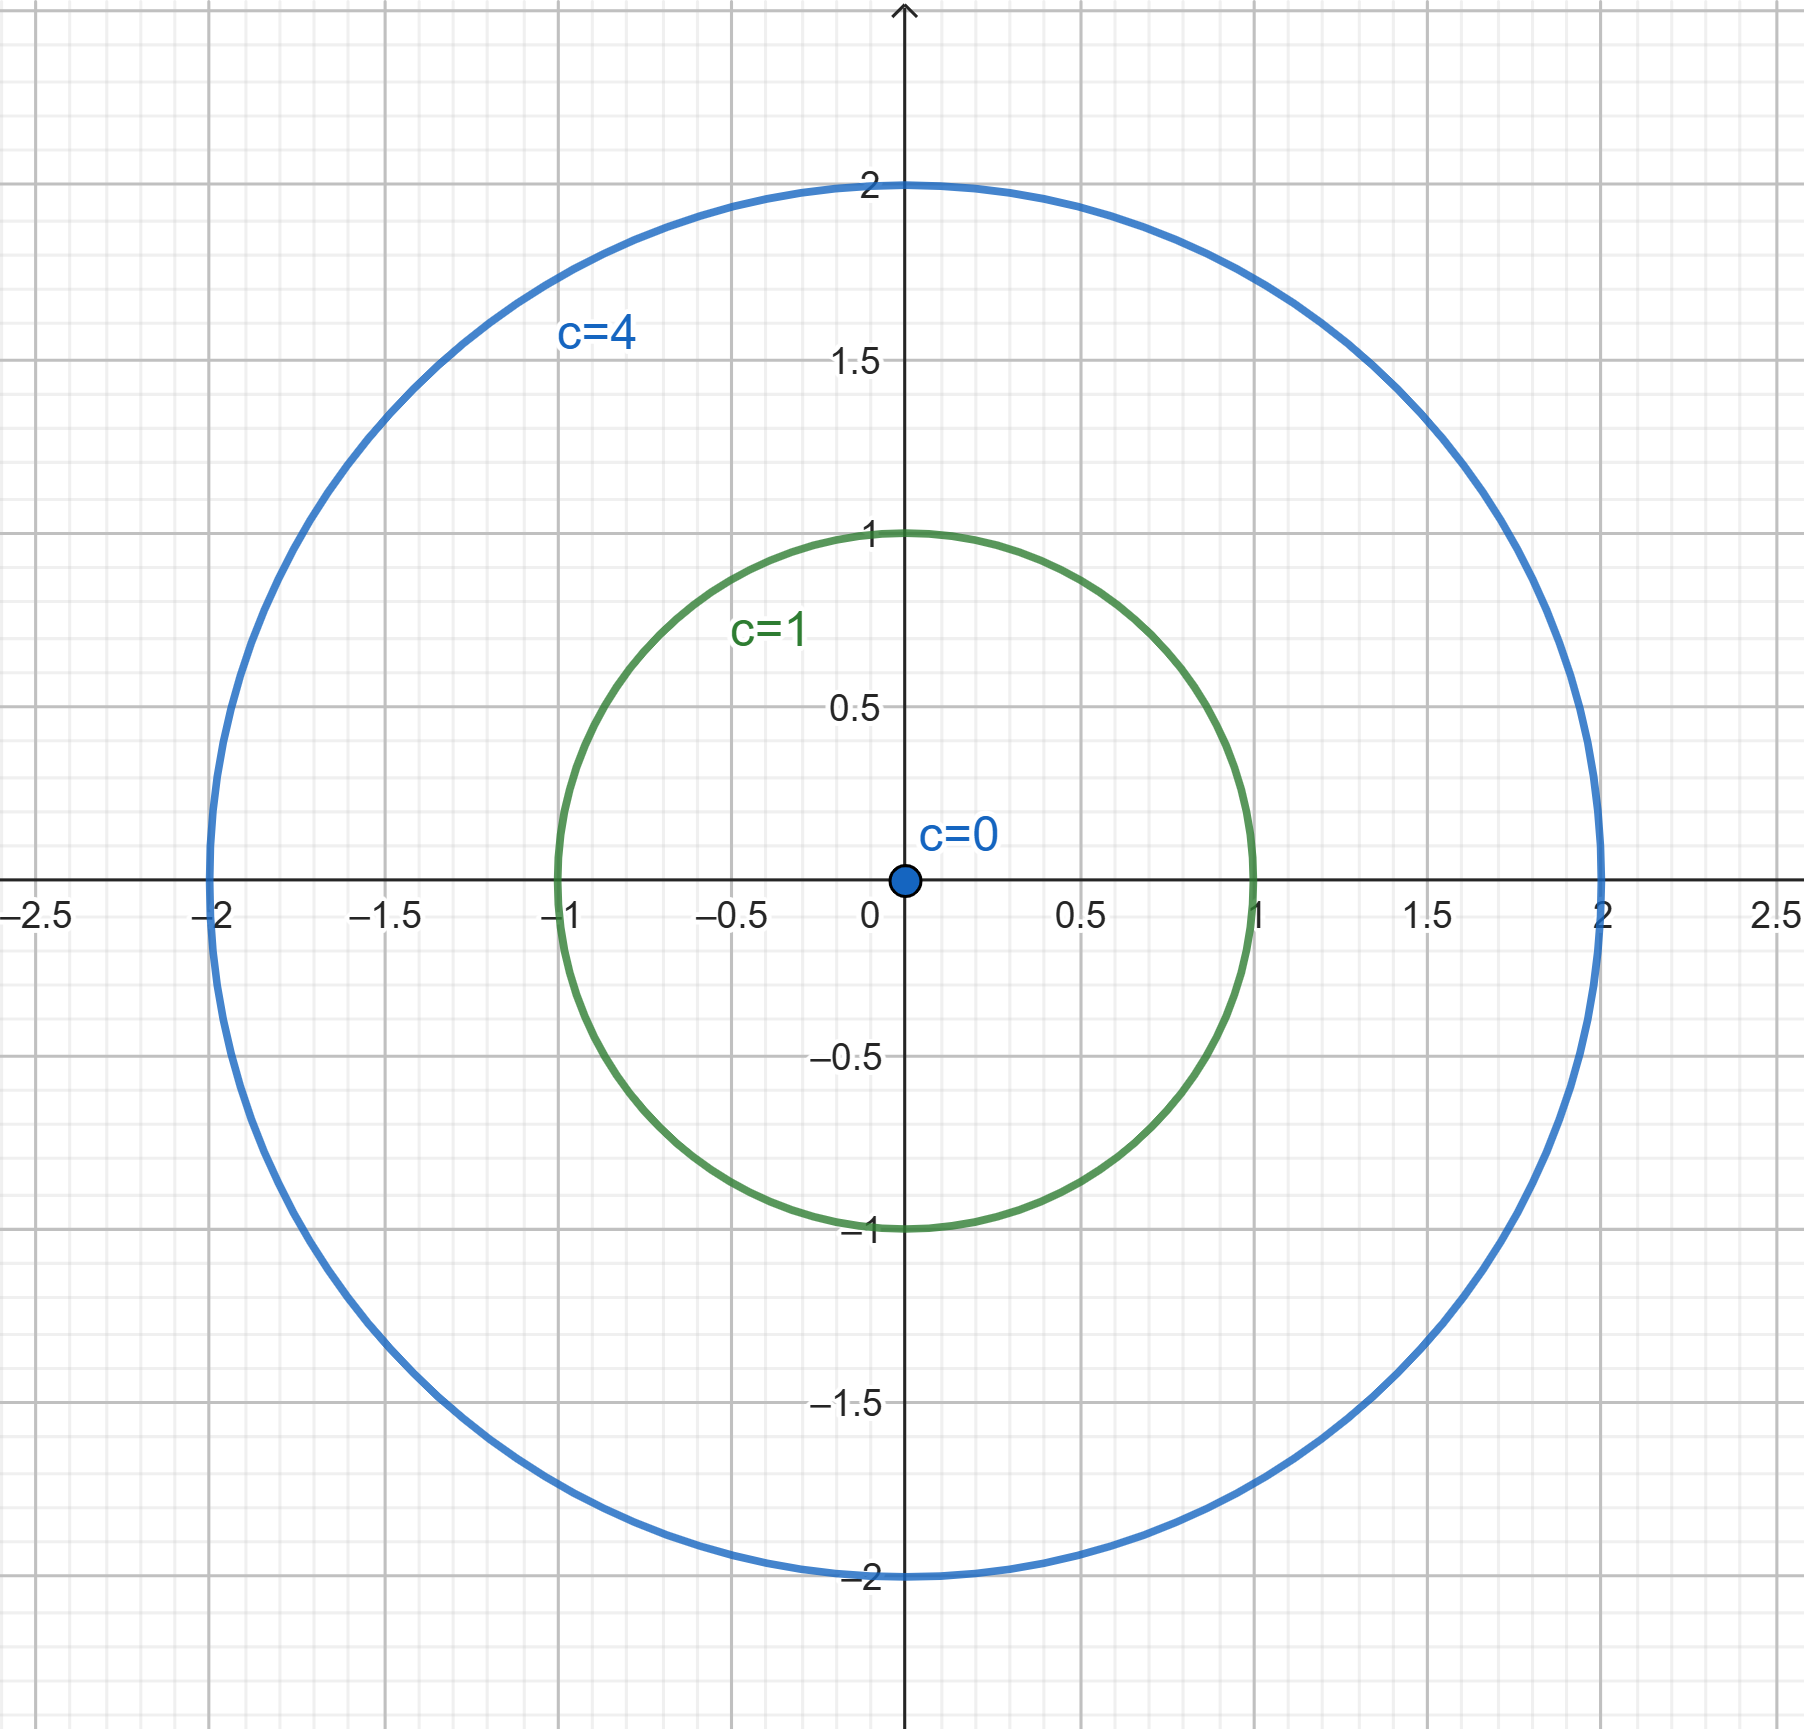
\includegraphics[width=0.5\textwidth]{../figs/conjunto1_r.png} % Cambia esta ruta por la ubicación de tu imagen
    \caption{Conjuntos de nivel}
    \label{fig:ejemplo} % Etiqueta para hacer referencia a la imagen
\end{figure}

En general, podemos determinar: 

   \[
        C(c,f)=
        \begin{dcases}
           \textnormal{Circunferencia centrada en (0,0) de radio} \sqrt{c},  & \textnormal{si}:  c>0 \\
(0,0)  & \textnormal{si}:\ c=0\\
\emptyset  & \textnormal{si}:\ c<0\\
        \end{dcases}
    \]

De esta manera, considerando la definicion de gráfica de una funcion, podemos representar la misma en $\Rn{3}$ tomando  la ecuacion del paraboloide: $z=x^2+y^2$

\begin{figure}[h!] % El entorno figure te permite incluir imágenes
    \centering
    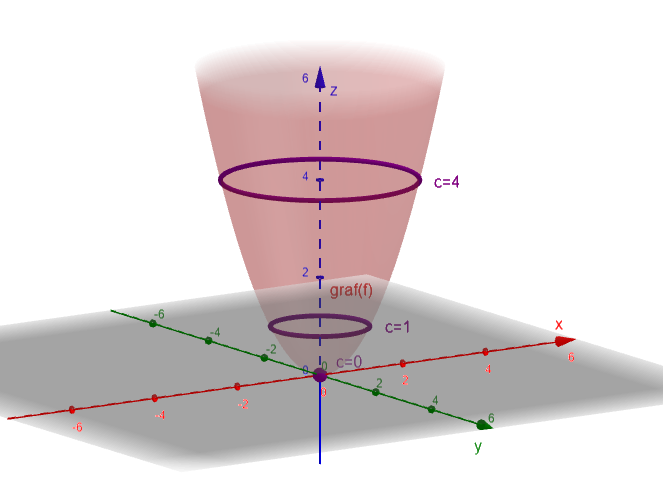
\includegraphics[width=0.5\textwidth]{../figs/conjunto1_r3.png} % Cambia esta ruta por la ubicación de tu imagen
    \caption{Conjuntos de nivel y graf(f)}
    \label{fig:ejemplo} % Etiqueta para hacer referencia a la imagen
\end{figure}



 

Ejemplo 2: Se toma la funcion $f(x,y)=\sqrt{x^2+y^2}$, donde empezamos a analizar los distintos conjuntos de nivel, tomando $c$ con diferentes constantes
 \[
C(0,f)=\{(x,y) \in U \backslash \sqrt{x^2+y^2}=0 \}
\]
 \[
C(1,f)=\{(x,y) \in U \backslash \sqrt{x^2+y^2}=1 \}
\]
 \[
C(2,f)=\{(x,y) \in U \backslash \sqrt{x^2+y^2}=2 \}
 \]

\begin{figure}[h!] % El entorno figure te permite incluir imágenes
    \centering
    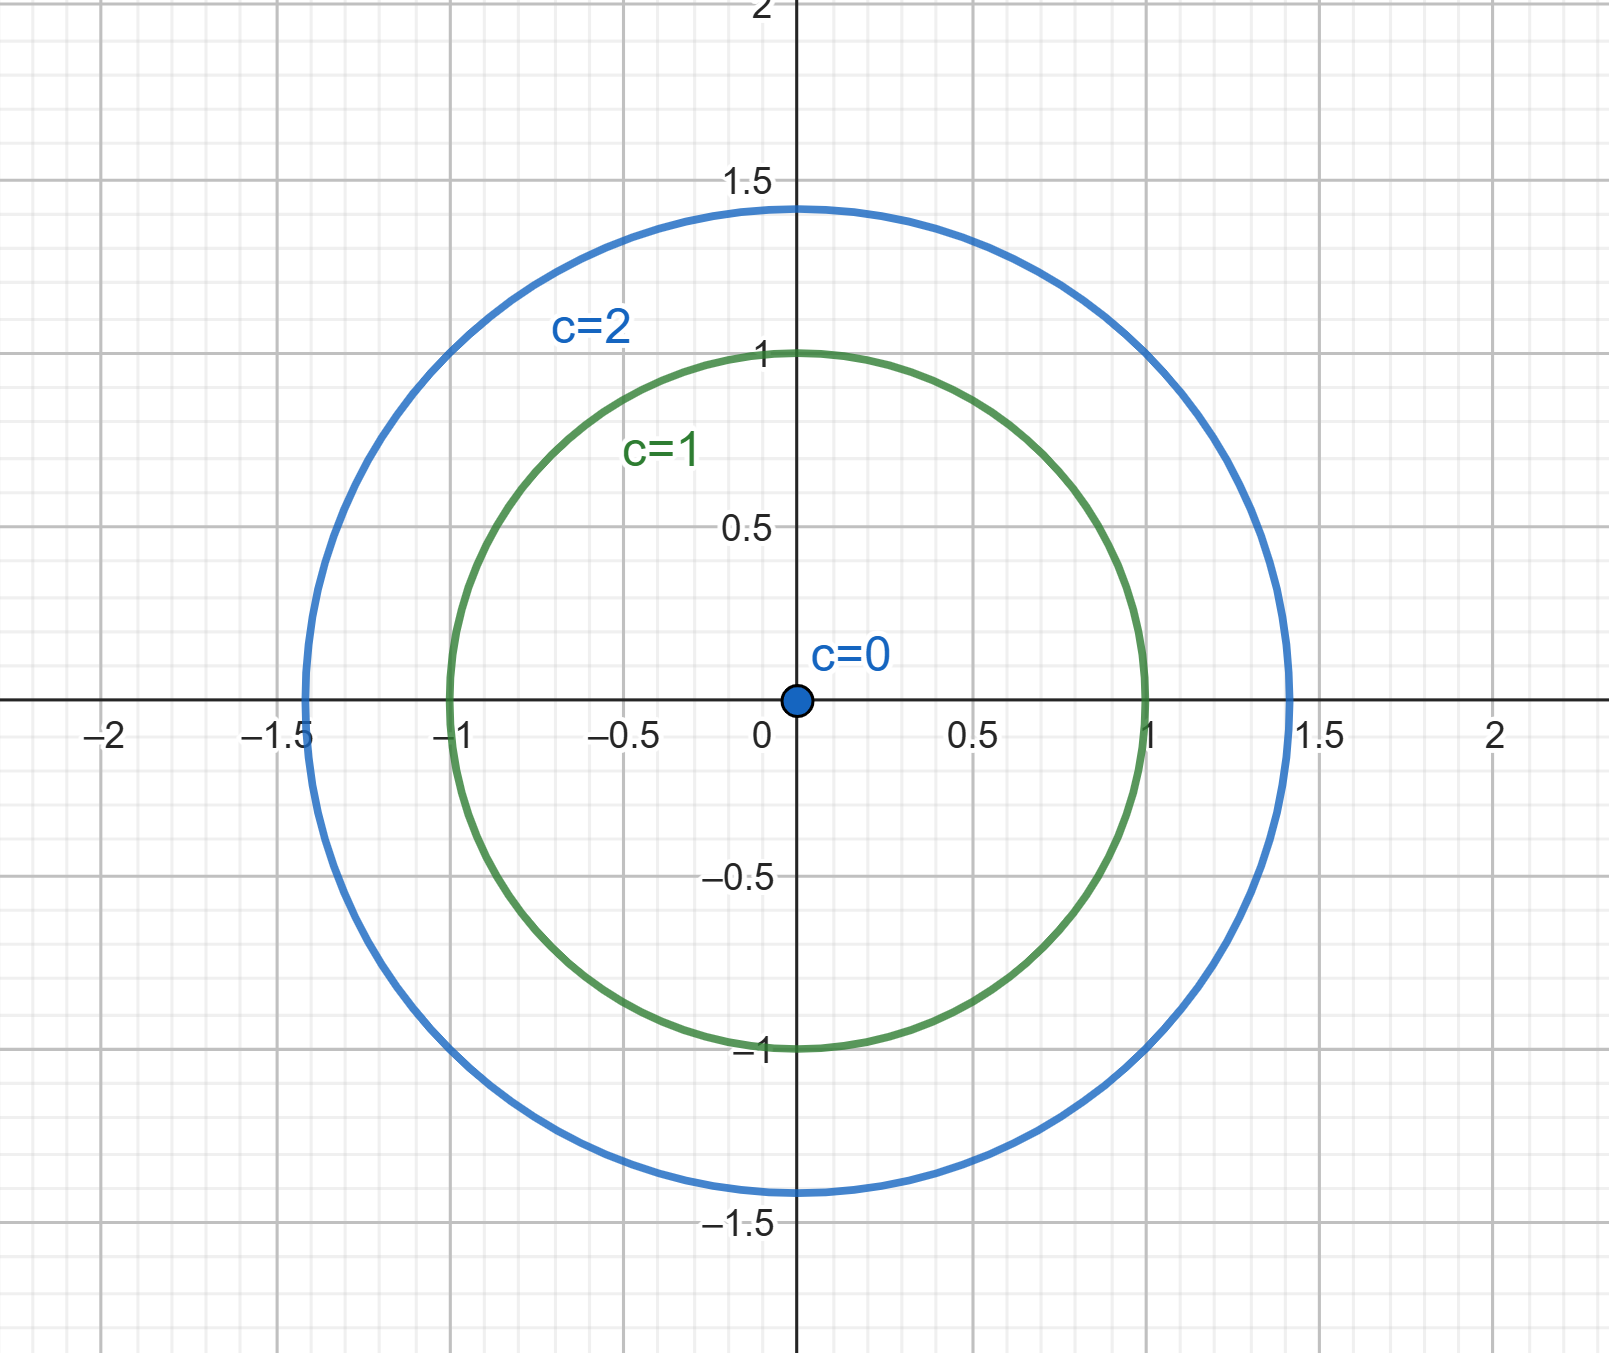
\includegraphics[width=0.5\textwidth]{../figs/conjunto2_r2.png} % Cambia esta ruta por la ubicación de tu imagen
    \caption{Conjuntos de nivel}
    \label{fig:ejemplo} % Etiqueta para hacer referencia a la imagen
\end{figure}

En general, podemos determinar: 

   \[
        C(c,f)=
        \begin{dcases}
           \textnormal{Circunferencia centrada en (0,0) de radio} c,  & \textnormal{si}:  c>0 \\
(0,0)  & \textnormal{si}:\ c=0\\
\emptyset  & \textnormal{si}:\ c<0\\
        \end{dcases}
    \]
\begin{figure}[h!] % El entorno figure te permite incluir imágenes
    \centering
    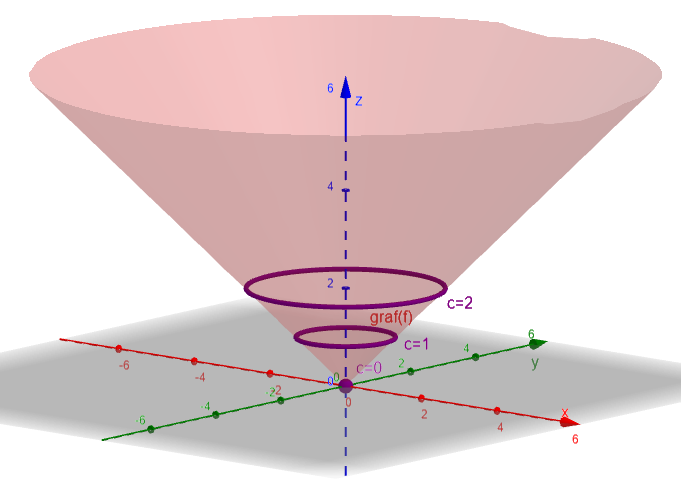
\includegraphics[width=0.5\textwidth]{../figs/conjunto2_r3.png} % Cambia esta ruta por la ubicación de tu imagen
    \caption{Conjuntos de nivel y graf(f)}
    \label{fig:ejemplo} % Etiqueta para hacer referencia a la imagen
\end{figure}

De esta manera, considerando la definicion de gráfica de una funcion, podemos representar la misma en $\Rn{3}$ tomando  la ecuacion de la parte superior de un cono: $z=\sqrt{x^2+y^2}$


Observacion: si tomaramos la ecuacion $z^2=x^2+y^2$ al despejar z obtenemos $|z|=\sqrt{x^2+y^2}$ obtendriamos que: 
 \[
        C(c,f)=
        \begin{dcases}
           \textnormal{Circunferencia centrada en (0,0) de radio} c,  & \textnormal{si}:  c>0 \\
(0,0)  & \textnormal{si}:\ c=0\\
\textnormal{Circunferencia centrada en (0,0) de radio} c,  & \textnormal{si}:\ c<0\\
        \end{dcases}
    \]

De esta manera, considerando la definicion de gráfica de una funcion, podemos representar la misma en $\Rn{3}$ tomando  la ecuacion del cono: $z^2=x^2+y^2$

\begin{figure}[h!] % El entorno figure te permite incluir imágenes
    \centering
    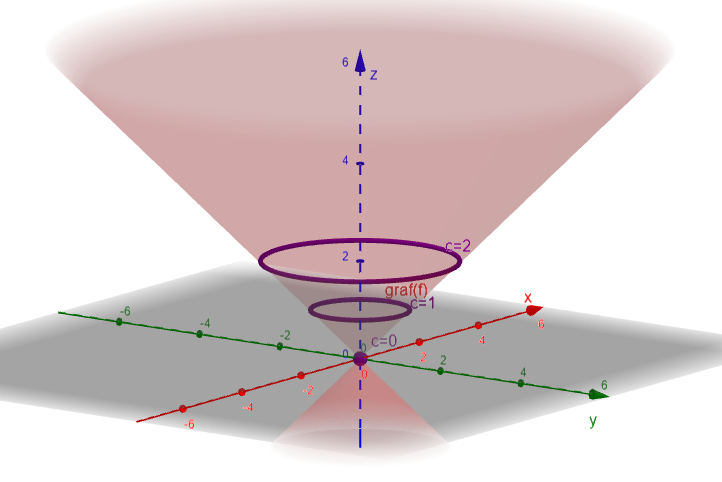
\includegraphics[width=0.5\textwidth]{../figs/conjunto3_r3.png} % Cambia esta ruta por la ubicación de tu imagen
    \caption{Conjuntos de nivel y graf(f)}
    \label{fig:ejemplo} % Etiqueta para hacer referencia a la imagen
\end{figure}


\end{definition}
